\let\negmedspace\undefined
\let\negthickspace\undefined
\documentclass[journal]{IEEEtran}
\usepackage[a5paper, margin=10mm, onecolumn]{geometry}
%\usepackage{lmodern} % Ensure lmodern is loaded for pdflatex
\usepackage{tfrupee} % Include tfrupee package

\setlength{\headheight}{1cm} % Set the height of the header box
\setlength{\headsep}{0mm}     % Set the distance between the header box and the top of the text

\usepackage{gvv-book}
\usepackage{gvv}
\usepackage{cite}
\usepackage{amsmath,amssymb,amsfonts,amsthm}
\usepackage{algorithmic}
\usepackage{graphicx}
\usepackage{textcomp}
\usepackage{xcolor}
\usepackage{txfonts}
\usepackage{listings}
\usepackage{enumitem}
\usepackage{mathtools}
\usepackage{gensymb}
\usepackage{comment}
\usepackage[breaklinks=true]{hyperref}
\usepackage{tkz-euclide} 
\usepackage{listings}
% \usepackage{gvv}                                        
\def\inputGnumericTable{}                                 
\usepackage[latin1]{inputenc}                                
\usepackage{color}                                            
\usepackage{array}                                            
\usepackage{longtable}                                       
\usepackage{calc}                                             
\usepackage{multirow}                                         
\usepackage{hhline}                                           
\usepackage{ifthen}                                           
\usepackage{lscape}
\begin{document}

\bibliographystyle{IEEEtran}
\vspace{3cm}

\title{10.3.6.2.2}
\author{EE24BTECH11058 - P.Shiny Diavajna}
% \maketitle
% \newpage
% \bigskip
{\let\newpage\relax\maketitle}

\renewcommand{\thefigure}{\theenumi}
\renewcommand{\thetable}{\theenumi}
\setlength{\intextsep}{10pt} % Space between text and floats


\numberwithin{equation}{enumi}
\numberwithin{figure}{enumi}
\renewcommand{\thetable}{\theenumi}
\textbf{Question:}\\
2 women and 5 men can together finish an embroidery work in 4 days, while 3 women and 6 men can finish it in 3 days. Find the time taken by 1 woman alone to finish the work, and also that taken by 1 man alone.\\

\textbf{Solution:}\\
Let the number of days taken by 1 woman alone to finish the work be $x$\\
Let the number of days taken by 1 man alone to finish the work be $y$\\

Then,\\
The amount of work done by a woman in 1 day is $\frac{1}{x}$\\
The amount of work done by a man in 1 day is $\frac{1}{y}$\\

Let,
\begin{align}
   \frac{1}{x} =p \text{ and } \frac{1}{y}=q
\end{align}

Then the equations are:
\begin{align}
    2p+5q=\frac{1}{4}\\
    3p+6q=\frac{1}{3}
\end{align}

\textbf{Matrix Form:}
\begin{align}
   \myvec{2 & 5 \\ 3 &6}\myvec{p\\q}= \myvec{\frac{1}{4}\\\frac{1}{3}}
\end{align}\\

\textbf{LU decomposition:}\\
For the system of linear equations $\vec{A}\vec{x}=\vec{b}$, if $\vec{A}$ is non-singular, we can decompose it as product $LU$ where $L$ is lower triangular matrix and $U$ is an upper triangular matrix.\\
The equation becomes 
\begin{align}
    \vec{LUx}=\vec{b} 
\end{align}
Taking 
\begin{align}
    \vec{y}=\vec{Ux}
\end{align}
Substituting (0.6) in (0.5)
\begin{align}
    \vec{Ly}=\vec{b}
\end{align}
We solve for $y$ in $\vec{L}\vec{y}=\vec{b}$ and then solve for $\vec{x}$ in $\vec{U}\vec{x}=\vec{y}$\\
Applying LU decomposition to matrix A, \\
For each column $j \geq k$, the entries of $U$ in the $k$th row are updated as:
\begin{align}
    U_{k,j} = A_{k,j} - \sum_{m=1}^{k-1} L_{k,m}.U_{m,j},   \forall{j \geq k}
\end{align}
For each row $i > k$, the entries of $L$ in the $k$th column are updated as:
\begin{align}
    L_{j,k} = \frac{1}{U_{k,k}}\brak{A_{j,k} - \sum_{m=1}^{k-1}.U_{m,k}}, \forall{i>k}
\end{align}
We find $\vec{L}$ and $\vec{U}$ as follows:
\begin{align}
    \vec{L}=\myvec{1 & 0\\ \frac{3}{2} & 1 } \\
    \vec{U}=\myvec{2 & 5\\ 0 & -\frac{3}{2} }
\end{align}
Solving $\vec{Ly}=\vec{b}$ by forward substitution,
\begin{align}
    \myvec{1 & 0 \\ \frac{3}{2}&1}\myvec{y_1\\y_2}&=\myvec{ \frac{1}{4} \\\frac{1}{3}}\\
    y_1&=\frac{1}{4}\\
    y_2&=-\frac{1}{24}\\
    y&=\myvec{\frac{1}{4}\\ -\frac{1}{24}}
\end{align}
Solving $\vec{Ux}=\vec{y}$
\begin{align}
    \myvec{2 & 5\\0 & -\frac{3}{2}}\myvec{p\\q}&=\myvec{\frac{1}{4}\\-\frac{1}{24}}\\
    p&=\frac{1}{18}\\
    q&=\frac{1}{36}
\end{align}
Hence, solution is
\begin{align}
    x=\frac{1}{p}=18\\
    y=\frac{1}{q}=36\\
    \myvec{x\\y}=\myvec{18\\36}
\end{align}

Therefore,\\
The time taken by 1 woman alone to finish the work is 18 days\\
The time taken by 1 man alone to finish the work is 36 days\\

\textbf{Plot:}\\
\begin{figure}[h]
   \centering
   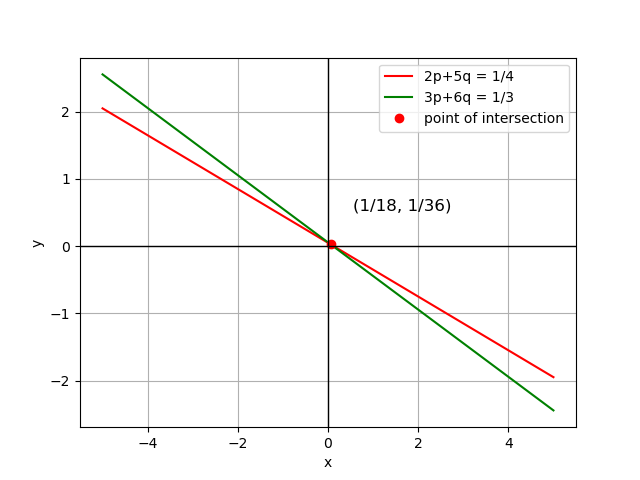
\includegraphics[width=\columnwidth]{figs/figure.png}
\end{figure}






\end{document}
